\documentclass[handout]{beamer}
 
\usepackage[utf8]{inputenc}
\usepackage{mathtools}
\usepackage{tikz}
\usetikzlibrary{calc}

\usetheme{CambridgeUS}
% \useoutertheme{split}
\setbeamertemplate{title page}[default][colsep=-4bp,rounded=true]

% only inlcude the current secition in the header
\AtBeginSection{
    \begin{frame}
        \tableofcontents[sections=\value{section}, sectionstyle=show/show]
    \end{frame}
}

%Information to be included in the title page:
\title{Digital Signatures}
\author{Rohit Musti}
\institute{CUNY - Hunter College}
\date{\today}
 
\begin{document}
 
\frame{\titlepage}

% Outline frame
\begin{frame}{Table of Contents}
  \tableofcontents
\end{frame}


\section{Overview}

\begin{frame}{Example Use Case}
    \begin{itemize}
        \item \pause Let's pretend you are a software company
        \item \pause Occasionally, you will distribute updates to your software
        \item \pause Customers will need a way to verify that the software is really from the company without sharing a secret key with every single customer
        \item \pause Enter digital signatures!
    \end{itemize}
\end{frame}

% Key Exchange Attqck
\begin{frame}{Digital Signatures Attack Game}
    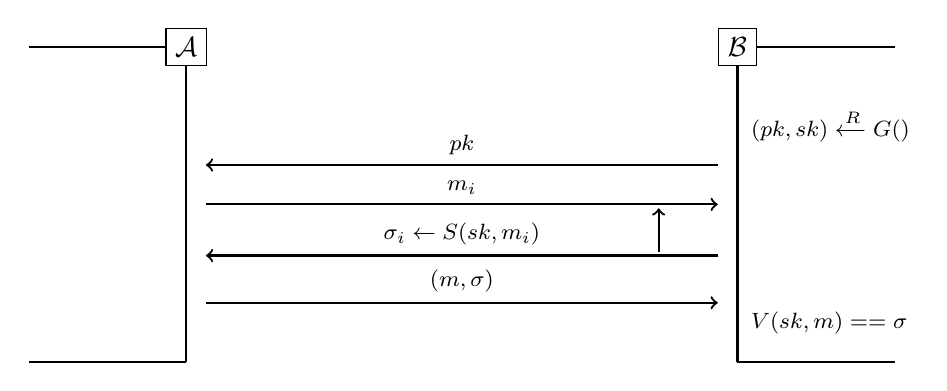
\begin{tikzpicture}
      \pause
        \node[draw] (AdversaryA) at (-3, 2) {\(\mathcal{A}\)}; 
        \draw[thick] (AdversaryA) -- ++(0, -4); 
        \draw[thick] (AdversaryA) -- ++(-2, 0);
        \draw[thick] (-3, -2) -- ++(-2, 0);
      \pause
        \node[draw] (ChallengerA) at (4,2) {\(\mathcal{B}\)}; 
        \draw[thick] (ChallengerA) -- ++(0, -4);
        \draw[thick] (ChallengerA) -- ++(2, 0);
        \draw[thick] (4, -2) -- ++(2, 0);

      \pause
        \node[draw=none,fill=none,anchor=west, font=\footnotesize] (choice0) at ($(ChallengerA) + (.05,-1)$) {\((pk, sk) \xleftarrow[]{R} G() \)};

      \pause
        \draw[->,thick] ($(ChallengerA)+(-0.25,-1.5)$) -- ($(AdversaryA)+(0.25,-1.5)$) node [pos=0.5,above,font=\footnotesize] {\(pk\)};

      \pause
        \draw[->,thick] ($(AdversaryA)+(0.25,-2)$) -- ($(ChallengerA)+(-0.25,-2)$) node [pos=0.5,above,font=\footnotesize] {\(m_i\)};

      \pause
        \draw[->,thick] ($(ChallengerA)+(-0.25,-2.65)$) -- ($(AdversaryA)+(0.25,-2.65)$) node [pos=0.5,above,font=\footnotesize] {\( \sigma_i \leftarrow S(sk, m_i) \)};

      \pause
        \draw[->,thick] ($(ChallengerA)+(-1,-2.6)$) -- ($(ChallengerA)+(-1,-2.05)$) node [pos=0.5,right,font=\footnotesize] {};

      \pause
        \draw[->,thick] ($(AdversaryA)+(0.25,-3.25)$) -- ($(ChallengerA)+(-0.25,-3.25)$) node [pos=0.5,above,font=\footnotesize] {\( (m,\sigma) \)};

      \pause
        \node[draw=none,fill=none,anchor=west, font=\footnotesize] (choice0) at ($(ChallengerA) + (.05,-3.5)$) {\(V(sk,m) == \sigma\)};

      \end{tikzpicture}
\end{frame}

\begin{frame}{Non-Repudiation}
    \begin{enumerate}
        \item \pause Non-Repudiation: there is no way to deny that the signature was not produced by someone with access to the secret key
        \item \pause This sounds legally useful right? Unfortunately not, it is very easy for someone to claim the public key isn't theirs or their secret key was exposed/leaked/stolen by a hacker.
        \item \pause Even more maliciously, Alice could have leaked her key right after or before sending a signatunre
    \end{enumerate}
\end{frame}

\begin{frame}{Limits}
    \begin{enumerate}
        \item \pause Binding Signatures: Easy for a signer to issue multiple yet contradicting signed messages
        \item \pause Duplicate Keys: Given a signature \(\sigma\) for a public key \(pk\), could I generate a \(pk', sk', m\) that produces \(\sigma' == \sigma\)
        \item \pause Future HW Queston: Is there an easy way to get around duplicate keys attacks???
    \end{enumerate}
\end{frame}

\section{Trapdoor Construction of Digital Signatures}

\begin{frame}{Construction}
    \pause
    \[S(sk, m) = y \leftarrow H(m), \sigma \leftarrow I(sk, y)\]
    \pause
    \[V(pk, m \sigma) = y \leftarrow F(pk, sigma), y == H(m)\]
\end{frame}

\begin{frame}{Security}
    \begin{itemize}
        \item \pause In order to prove security we most model the hash function as a random oracle
        \item \pause This means that \(y\) is essentially a random point in the space, and there is no way for an attacker to forge its signature
        \item \pause Without this hashing, an attacker could trivially generate secure signatures! Future HW question: How???
    \end{itemize}
\end{frame}

\end{document}